\documentclass[a4paper,12pt]{article}
\usepackage{graphicx}
\usepackage{amsmath}
\usepackage{hyperref}
\usepackage{amsfonts}
\usepackage{geometry}
\usepackage{float}

\geometry{a4paper, margin=1in}

\title{Prepoznavanje registrskih tablic z uporabo strojnega učenja}
\author{Miha Štih (89221324), Luka Uršič (89221145)}
\date{}

\begin{document}

\maketitle

\section*{Repozitorij projekta}
\url{https://github.com/urluur/Registration-Plate-Recognition}

\section*{Cilj projekta}
Cilj najinega projekta je bil razviti sistem za prepoznavanje in identifikacijo avtomobilskih tablic iz slik. Delovati bi moral tako, da bi mu dali sliko, program pa bi v primeru, da je na sliki uspel najti avtomobilsko tablico, vrnil registrsko številko s tablice in označil lokacijo tablice na sliki.

\section*{Izvedba projekta}
Projekt sva začela tako, da sva najprej izbrala dataset, ki ga bova uporabila za projekt. Izbrala sva si dataset \textit{“Car License Plate Detection”} z spletne strani Kaggle. Kot se je pozneje izkazalo, nisva izbrala najbolj optimalnega dataseta, saj je bil ta sestavljen iz samo 433 slik avtomobilov, kar pa je premalo, da bi se najin model lahko dobro naučil.

Ker so bile slike dataseta ločene od podatkov, sva začela z zbiranjem podatkov. S tem namenom sva pripravila \texttt{utils.py} datoteko, ki vsebuje 3 različne funkcije za ekstrakcijo podatkov, saj so bili relevantni podatki podani v XML datotekah za vsako izmed slik posebej. Tako torej pridobimo \texttt{bbox} podatke iz XML datotek oziroma \texttt{xmin}, \texttt{xmax}, \texttt{ymin}, in \texttt{ymax}, ki določijo kote pravokotnika avtomobilske tablice na sliki. Za pretvorbo slik v uporabne podatke pa sva uporabila \texttt{numpy}.

\subsection*{Uporaba OpenCV in Pytesseract}
Ko so funkcije za pridobitev podatkov delovale, sva poskusila uporabiti OpenCV orodje za manipulacijo s slikami. Naučila sva se, kako se bere slike, kako riše pravokotnik in kako lahko napiševa številke tablice kot tekst na sliko. Poskusila sva uporabiti tudi \texttt{pytesseract} knjižnico, ki uporablja Googlov Tesseract OCR Engine za branje teksta iz slik in jo tudi uporabljala skoraj do končne verzije projekta.

\pagebreak

\subsection*{Delitev podatkov in učenje modela}
Nato sva uporabila funkcijo \texttt{train\_test\_split} iz \texttt{scikit-learn} knjižnice za naključni split podatkov na tiste, ki bodo uporabljeni za učenje in tiste, katere bova uporabila za testiranje. Za velikost test seta sva izbrala samo 15\% od vseh podatkov, saj je bil izbran dataset že tako ali tako majhen, tako da nama ostane čim več podatkov za učenje modela.

\subsection*{Model in transformacija slik}
Najin naslednji korak je bil sestavljanje in učenje modela na datasetu. Za to sva uporabila \texttt{keras}, saj je preprost za uporabo. Kot model sva izbrala najpreprostejšo verzijo \texttt{Sequential} in dodala nekaj slojev. Najin model je narejen tako, da poskuša napovedati lokacije pravokotnika, kjer naj bi bila avtomobilska tablica (lokacijo na sliki). Začela sva z tem, da sva slike transformirala do velikosti 224x224px in učila model z naslednjimi sloji.

\begin{figure}[H]
    \centering
    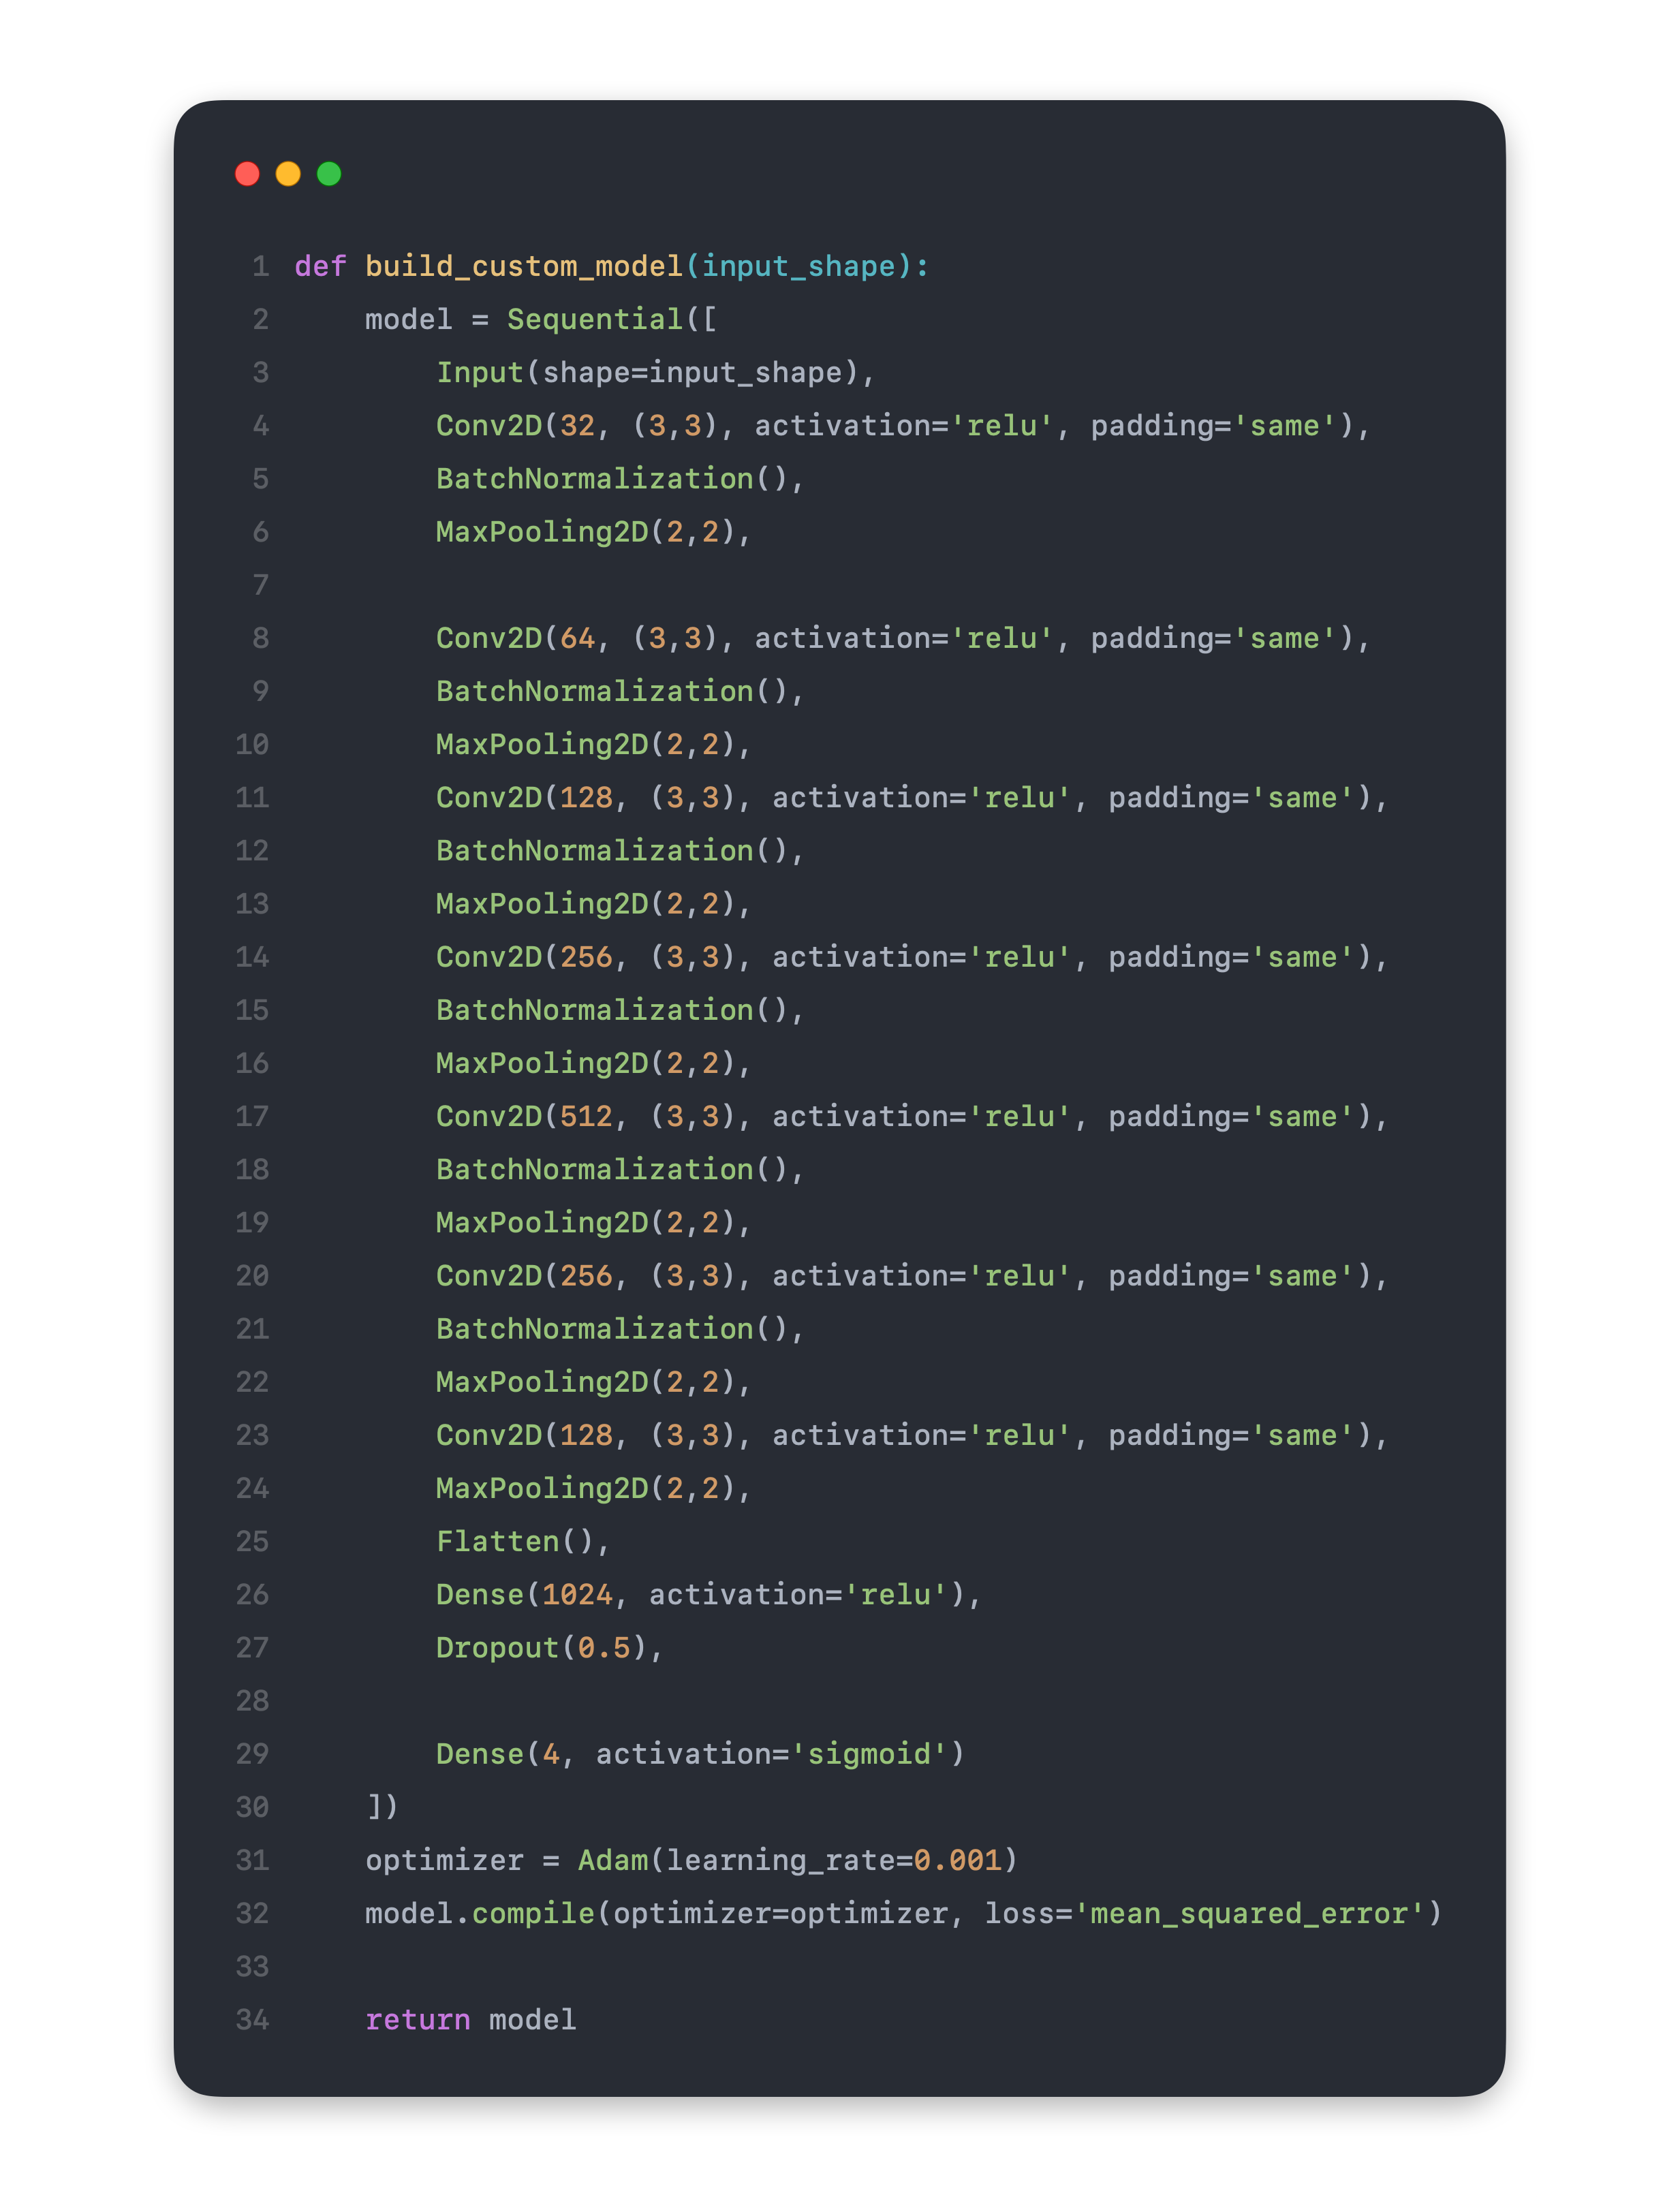
\includegraphics[width=0.7\textwidth]{img/build_custom_model1.png}
    \caption{Začetna sestava modela}
\end{figure}

\subsection*{Izboljšave modela}
Ker nama model ni dal želenih rezultatov, sva poskusila več različnih kombinacij slojev in \texttt{loss} funkcij, kot nama je priporočil asistent. Izkazalo se je, da nama \texttt{mean\_squared\_error} še vedno daje najboljše rezultate. Poskusila sva še \texttt{IoULoss} in \texttt{GIoULoss}, a se nobena ni izkazala bolje kot \texttt{mean\_squared\_error}.

Struktura slojev se je medtem spremenila v naslednje:

\begin{figure}[H]
    \centering
    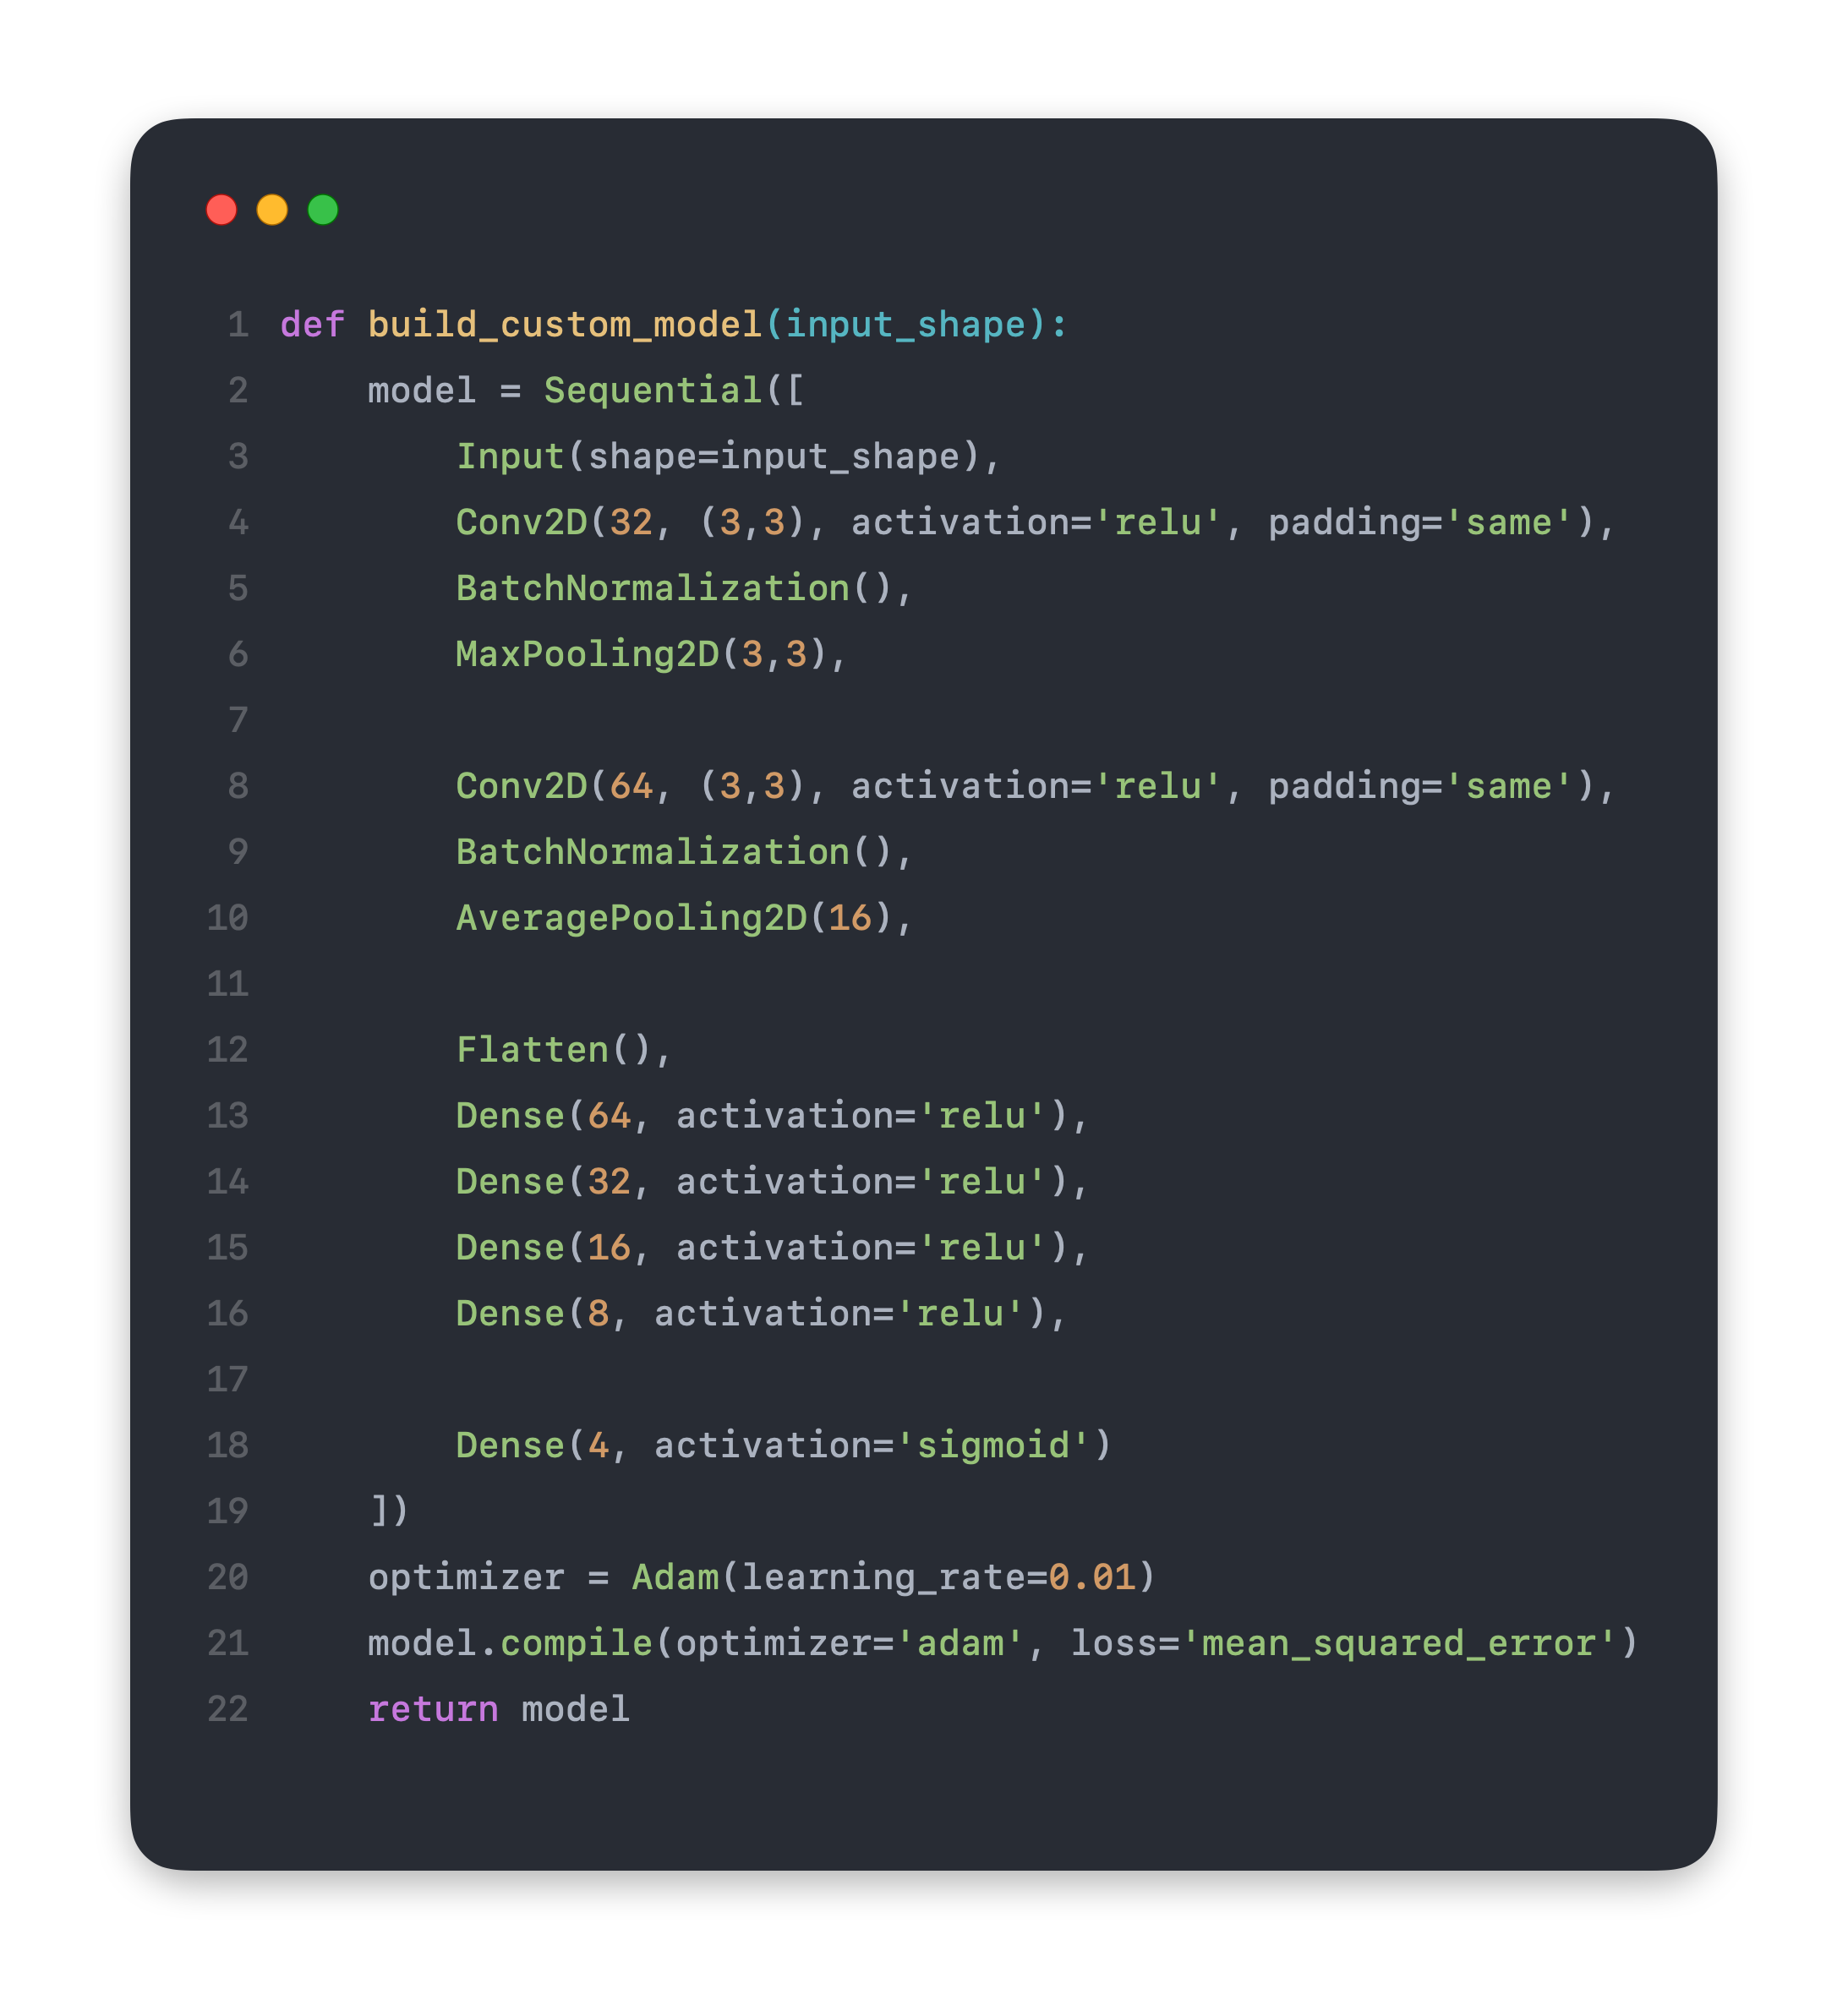
\includegraphics[width=0.8\textwidth]{img/build_custom_model2.png}
    \caption{Končna sestava modela}
\end{figure}

Za boljše učenje sva tudi spremenila velikost slik, ki jih uporabiva za učenje in torej iz 224x224px v 500x500px, kar misliva da je malce pomagalo.

Med ugibanjem slojev pa sva napisala še funkcijo \texttt{load\_and\_predict}. Deluje tako, da najprej pretovori podano sliko v pravilno velikost, torej 500x500px in nato preko prej omenjenega modela poskuša najti lokacijo avtomobilske tablice. Ko lokacijo oz pravokotnik najde, pretvori sliko v črno-belo in uporabi pytesseract OCR za prepoznavo znakov z tega dela slike. Za vsak slučaj pa sva dodala še nekaj maneverskega prostora tako da prebere sliko, ki je na vsako stran za 10px večja od pravokotnika.

Po nekaj preizkusih modela sva na primeru dobila naslednji rezultat:

\begin{figure}[H]
    \centering
    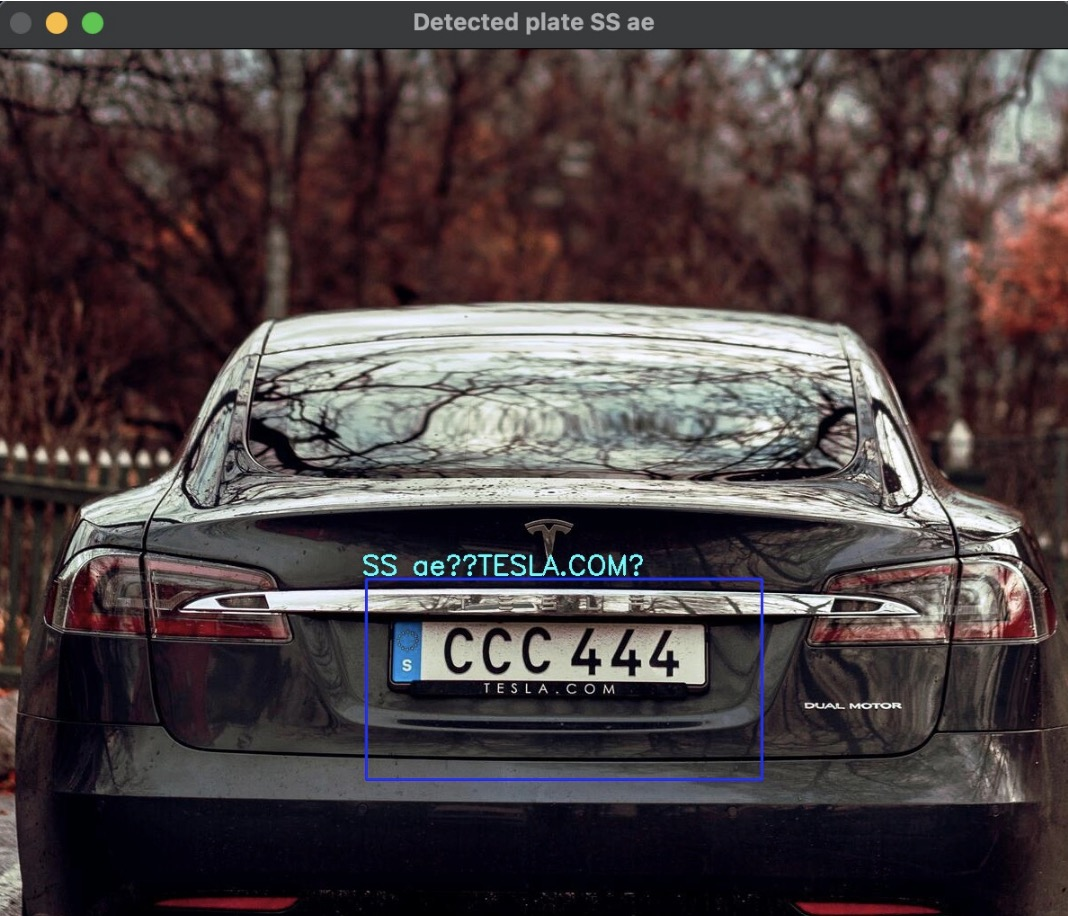
\includegraphics[width=0.65\textwidth]{img/plate_detection1.jpg}
    \caption{Začetna zaznava tablice}
\end{figure}

Kar nama je pokazalo, da prepoznavanje lokacije tablic vsaj približno deluje, medtem ko OCR ne deluje tako kot bi moral. Ker OCR ni deloval po pričakovanjih sva se odločila da ga raje zamenjava z EasyOCR, ki se je izkazal dosti bolje in sedaj bere tablice kot bi moral. To je lahko vidno na spodnji sliki (v primerjavi z prejšnjo sliko).

\begin{figure}[H]
    \centering
    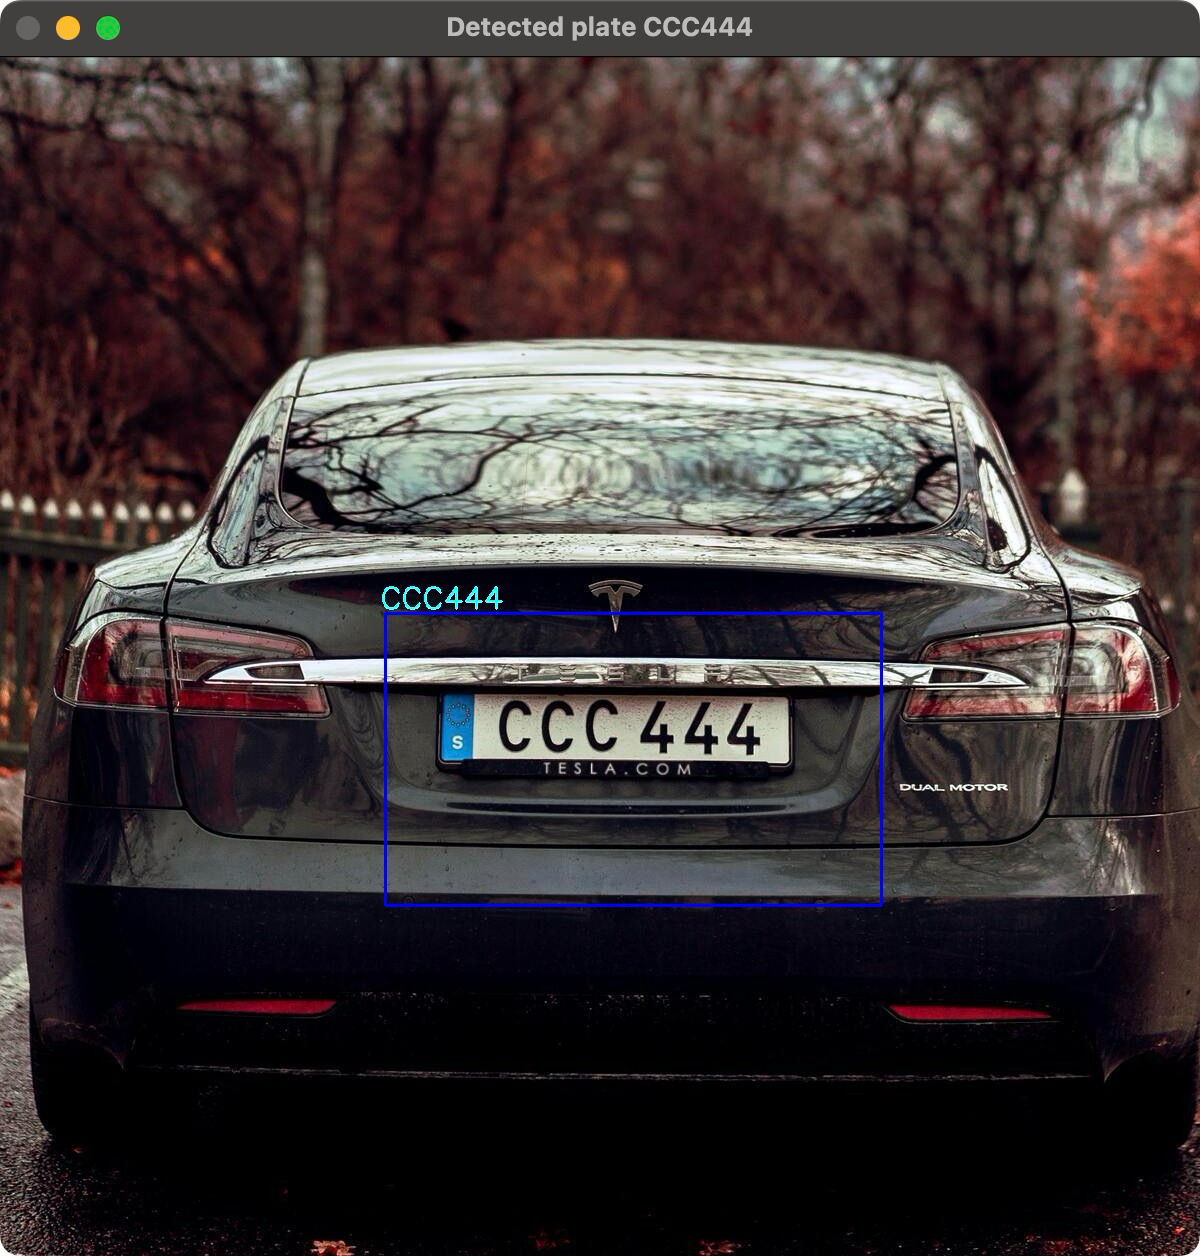
\includegraphics[width=0.65\textwidth]{img/plate_detection2.jpg}
    \caption{Končna zaznava tablice}
\end{figure}

\section*{Nadgradnje}

Ker je na tej točki projekt deloval kot bi moral je bil premaknjen iz navadnih python
datotek v Jupyter notebook, da se ga bo dalo lažje uporabljati ter nadgrajevati.

Kot dodatno sva uporabila tudi sklearn in matplotlib knjižnici za lepši prikaz delovanja
najinega modela. Prikazani so Confusion Matrix, graf napačno pozitivnih v primerjavi
z pravilnimi in graf točnosti.

Za konec je Luka že začel s prvo dejansko nadgradnjo, ki omogoča, da programu ni
treba podati slike avtomobila, pač pa lahko z uporabo kamere tablice beremo v
realnem času.

\section*{Zaključek}
Projekt naju je malo presenetil, saj je bil težji od pričakovanj za izvedbo. Ker še vedno ne deluje optimalno kot predvideno, misliva, da obstaja nekaj možnih izboljšav. Poudarek bi dala na zamenjavo dataseta, kot nama je svetoval že asistent. Trenutno uporabljen dataset je premajhen, da bi se model učinkovito naučil iskati lokacije tablic na slikah in bi bil tako večji dataset več kot dobrodošel.

Skratka, vidiva tudi več
drugih možnih izboljšav in nadgradenj za projekt, saj ima potencialno veliko praktično
uporabnost na več različnih področjih. Vse od nadzora prometa pa do parkirišč in
radarjev.

\section*{Povezave/viri}
\begin{itemize}
    \item \href{https://www.kaggle.com/datasets/andrewmvd/car-plate-detection}{Uporabljen dataset}
    \item \href{https://opencv.org/}{OpenCV}
    \item \href{https://pypi.org/project/pytesseract/}{Pytesseract}
    \item \href{https://keras.io/api/keras\_cv/losses/}{Keras losses}
    \item \href{https://scikit-learn.org/stable/modules/generated/sklearn.model\_selection.train\_test\_split.html}{Train\_test\_split funkcija}
    \item \href{https://numpy.org/}{Numpy}
    \item \href{https://github.com/JaidedAI/EasyOCR}{EasyOCR}
    \item \href{https://matplotlib.org/}{MatPlotLib}
    \item \href{https://www.datacamp.com/tutorial/python-xml-elementtree}{XML parsing}
\end{itemize}

\end{document}